\documentclass{article}
\usepackage[utf8]{inputenc}
\usepackage[fleqn]{amsmath}
\usepackage[T1]{fontenc}
\usepackage{parskip}
\usepackage{booktabs}
\usepackage{amsmath,amssymb,amsfonts}
\usepackage{natbib}
\usepackage{textcomp}
\usepackage{booktabs}
\usepackage{pgfplots}
\usepackage{pgfplotstable}
\usepackage{array}
\usepackage{bbold}
\usepackage{amssymb}
\usepackage[procnames]{listings}
\usepackage{color}
\usepackage{graphicx}

\addtolength{\oddsidemargin}{-.875in}
\addtolength{\evensidemargin}{-.875in}
\addtolength{\textwidth}{1.75in}

\addtolength{\topmargin}{-.875in}
\addtolength{\textheight}{1.75in}

\makeatletter
\newcommand{\distas}[1]{\mathbin{\overset{#1}{\kern\z@\sim}}}%
\newsavebox{\mybox}\newsavebox{\mysim}
\newcommand{\distras}[1]{%
	\savebox{\mybox}{\hbox{\kern3pt$\scriptstyle#1$\kern3pt}}%
	\savebox{\mysim}{\hbox{$\sim$}}%
	\mathbin{\overset{#1}{\kern\z@\resizebox{\wd\mybox}{\ht\mysim}{$\sim$}}}%
}
\makeatother

\title{Gamma approximation of Log Normal distribution for Ricker Map Inference}
\author{Raphael Lopez Kaufman}
\date{}

\begin{document}


\section*{Bootstrap filter}
In order to test a Python implementation of the bootstrap filter(which can be found here: https://github.com/rlk-ama/dissertation/bootstrap-filter/filter.py) we used the following simple model:
\begin{equation*}
X_t = \phi X_{t-1} + V_t
\end{equation*}
\begin{equation*}
Y_t = X_t + W_t
\end{equation*}
where $V_t, W_t \distas{iid} \mathcal{N} (0,1)$ and $\phi=0.95$.\\
We compared the values of $\mathrm{E}[X_t|y_{0:t}]$ given by our implementation and the ones given by a Kalman filter (package KalmanFilter of library pykalman) for 100 time steps and 100 particles. We also calculated the ESS as shown in Figure~\ref{fig:bootstrap}.

\begin{figure}[htb]
	\centering
	\begin{minipage}{.45\textwidth}
		\centering
		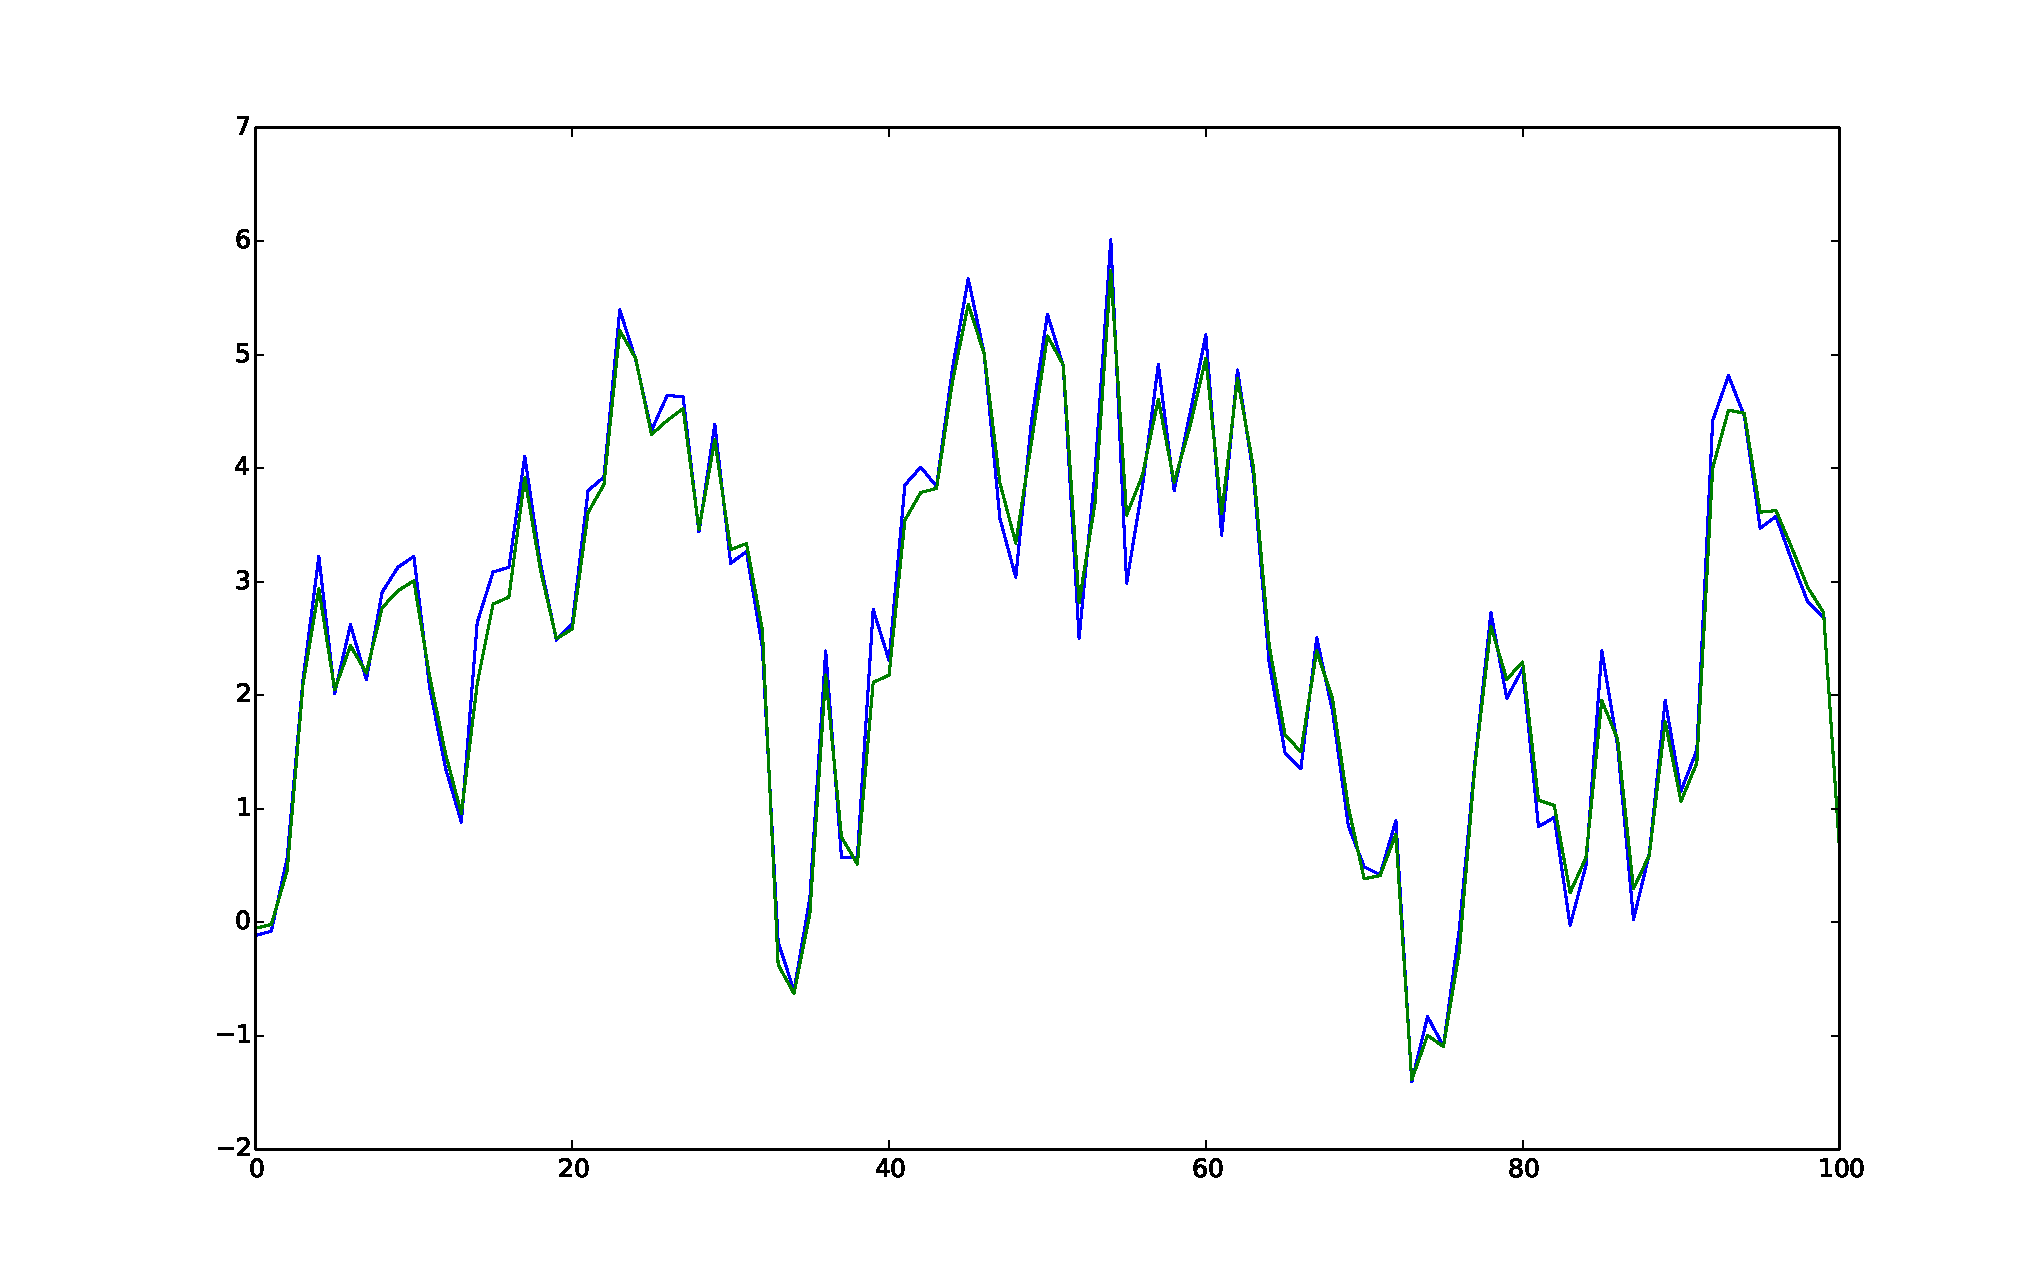
\includegraphics[width=0.97\linewidth]{bootstrap-filter/verif_filter.pdf}
	\end{minipage}
	\begin{minipage}{.45\textwidth}
		\centering
		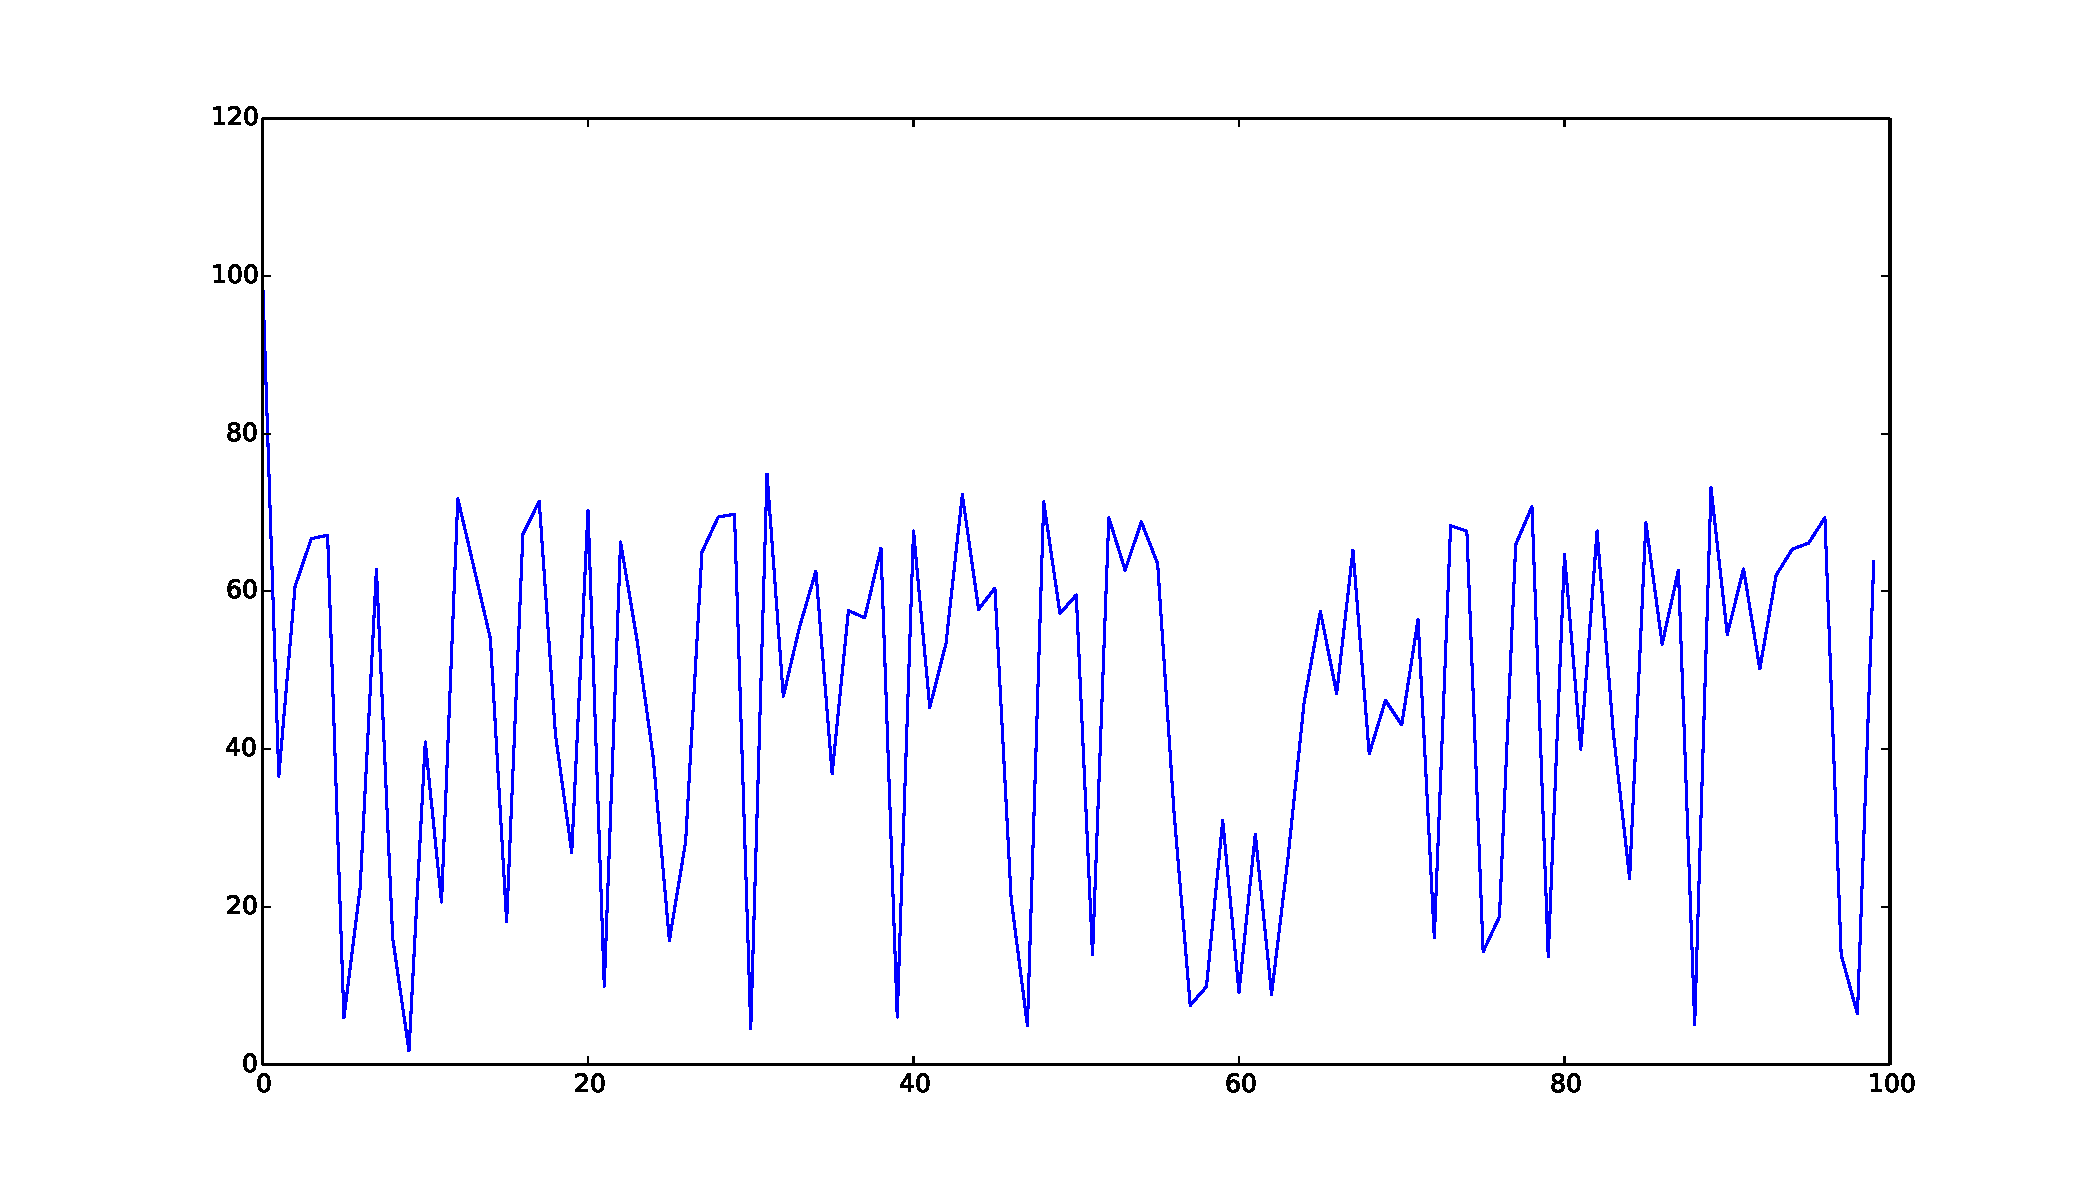
\includegraphics[width=0.97\linewidth]{bootstrap-filter/ESS_filter.pdf}
	\end{minipage}
	\caption{\textbf{(left)} Comparison of the expected value of the filtering distribution obtained using the Python implementation of the bootstrap filter \textbf{(blue)} and a Kalman filter \textbf{(green)}. \textbf{(right)} The ESS for the Python implementation of the bootstrap filter. }
	\label{fig:bootstrap}
\end{figure}

\section*{Gamma approximation to Log-Normal distribution}
The Ricker Map is the following model:
\begin{equation*}
N_t = rN_{t-1}e^{-N_{t-1}}e^{Z_t}
\end{equation*}
\begin{equation*}
Y_t \sim Poisson(\phi N_t)
\end{equation*}
where $Z_t \sim \mathcal{N} (0,\sigma^2)$.\\
Therefore $N_t \sim \log\mathcal{N} (\log{(rN_{t-1}e^{-N_{t-1}})},\sigma^2)$. To approximate a Log-normal distribution we tried to minimize the Kullback-Leibler divergence from a Gamma to a Log-normal, ie we tried to minimize:
\begin{equation*}
D_{KL}(P||Q)(\alpha, \theta) = \int_{0}^{\infty}{p(z|\mu, \sigma^2)\log(\frac{p(z|\mu, \sigma^2)}{q(z|\alpha, \theta)})\mathrm{d}z}
\end{equation*}
where $p$ is the probability density function of a $\log\mathcal{N}(\mu, \sigma^2)$ and $q$ of a Gamma with shape $\alpha$ and scale $\theta$
We have:
\begin{equation*}
D_{KL}(P||Q)(\alpha, \theta) = C + \alpha\log(\theta) + \log(\Gamma(\alpha)) - \alpha\mathrm{E_p}[\log(Z)] + \frac{1}{\theta}\mathrm{E_p}[Z]
\end{equation*}
Therefore:
\begin{equation*}
\frac{\partial }{\partial \alpha}(D_{KL}(P||Q)) = \log(\theta) + \psi^{(0)}(\alpha)-\mathrm{E_p}[\log(Z)]
\end{equation*}
\begin{equation*}
\frac{\partial }{\partial \theta}(D_{KL}(P||Q)) = \frac{\alpha}{\theta} - \frac{1}{\theta^2}\mathrm{E_p}[Z]
\end{equation*}
where $\psi^{(0)}$ is the digamma function.
\clearpage
Since $\mathrm{E_p}[\log(Z)]=\mu$ and $\mathrm{E_p}[Z] = e^{\mu+\frac{\sigma^2}{2}}$, we finally have that, setting the partial derivatives to zero:
\begin{equation*}
\alpha=e^{\psi^{(0)}(\alpha)+\frac{\sigma^2}{2}}
\end{equation*}
\begin{equation*}
\theta=\frac{1}{\alpha}e^{\mu+\frac{\sigma^2}{2}}
\end{equation*}
If we take $\psi^{(0)}(\alpha) \approx \log(\alpha)-\frac{1}{2\alpha}$ we finally have $\alpha =\frac{1}{\sigma^2}$ and $\theta=\frac{1}{\alpha}e^{\mu+\frac{\sigma^2}{2}}$.
In our case we will thus approximate the distribution of $N_t$ by
\begin{equation*}
q(n_t|\alpha(n_{t-1}), \theta(n_{t-1})) = Gamma(\ \cdot \ ; \alpha(n_{t-1}), \theta(n_{t-1}) )
\end{equation*}
where $ \alpha(n_{t-1})= \frac{1}{\sigma^2}$ and $\theta(n_{t-1})=\sigma^2e^{\log(rn_{t-1}e^{n_{t-1}})+\frac{\sigma^2}{2}}$, since $\mu = 0$.\\
Therefore our proposal for the bootstrap filter will be the following:
\begin{equation*}
\begin{split}
q_{t|t-1}(n_t|n_{t-1}, y_t) & \propto  p(y_t|n_t)q(n_t|n_{t-1}) \\
& \propto e^{-\phi n_t}(\phi N_t)^{y_t}n_t^{\alpha(n_{t-1})-1}e^{-\frac{n_t}{\theta(n_{t-1})}}
\end{split}
\end{equation*}
ie:
\begin{equation*}
q_{t|t-1}(n_t|n_{t-1}, y_t) = Gamma(\ \cdot \ ; y_t+\alpha(n_{t-1}), \frac{\theta(n_{t-1})}{\theta(n_{t-1})\phi + 1})\end{equation*}
Simulation carried out with $\log(r)=2.5$, $\phi=10$ and $\sigma=0.3$. We also set $N_0 \sim Gamma(3,1)$ in order to have $N_0$ around 3-4. A value of 3.8 as in Wood's paper for $\log(r)$ gave underflow and overflows in the Python code. Figure~\ref{fig:prior} shows results with prior proposal and Figure~\ref{fig:gamma} with gamma proposal.

\begin{figure}[htb]
	\centering
	\begin{minipage}{.45\textwidth}
		\centering
		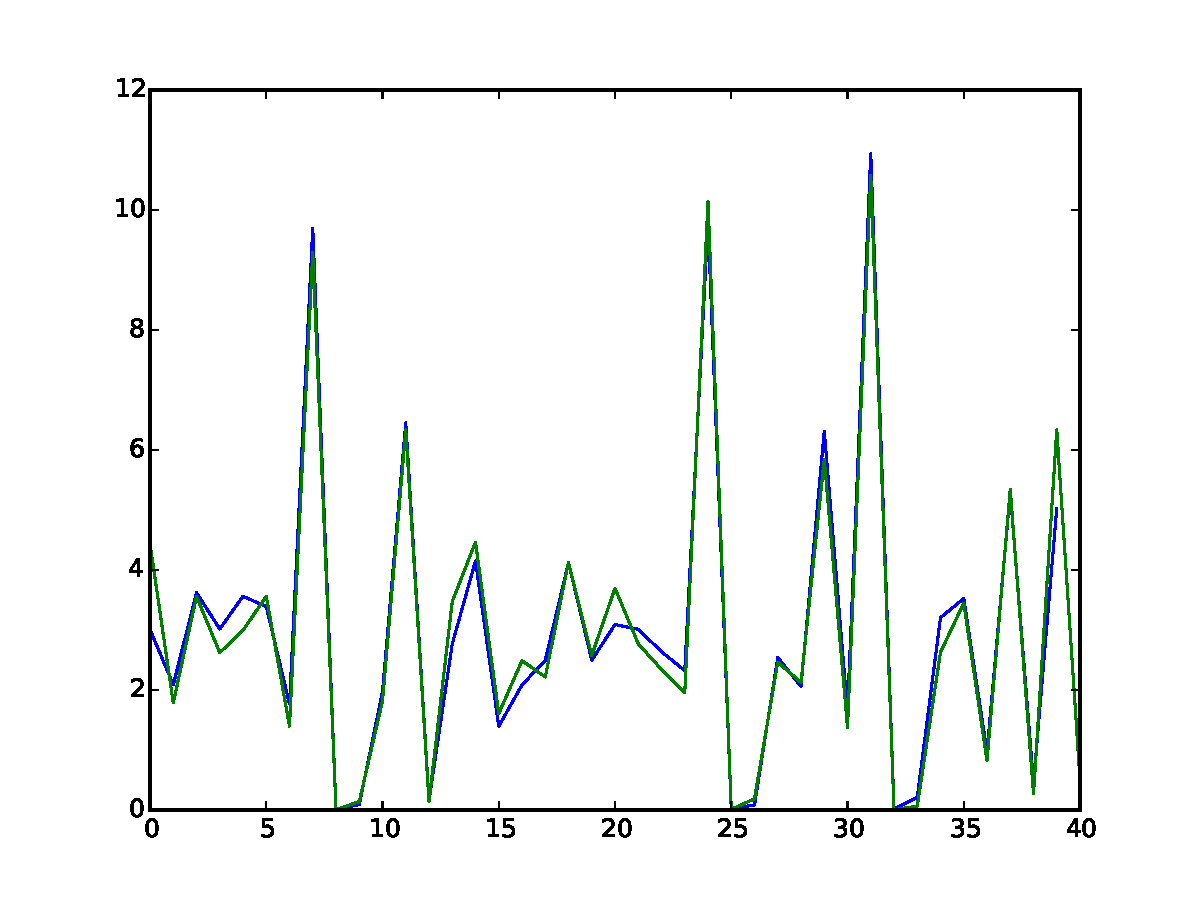
\includegraphics[width=0.97\linewidth]{/home/raphael/dissertation/bootstrap-filter/diagno_prior.pdf}
	\end{minipage}
	\begin{minipage}{.45\textwidth}
		\centering
		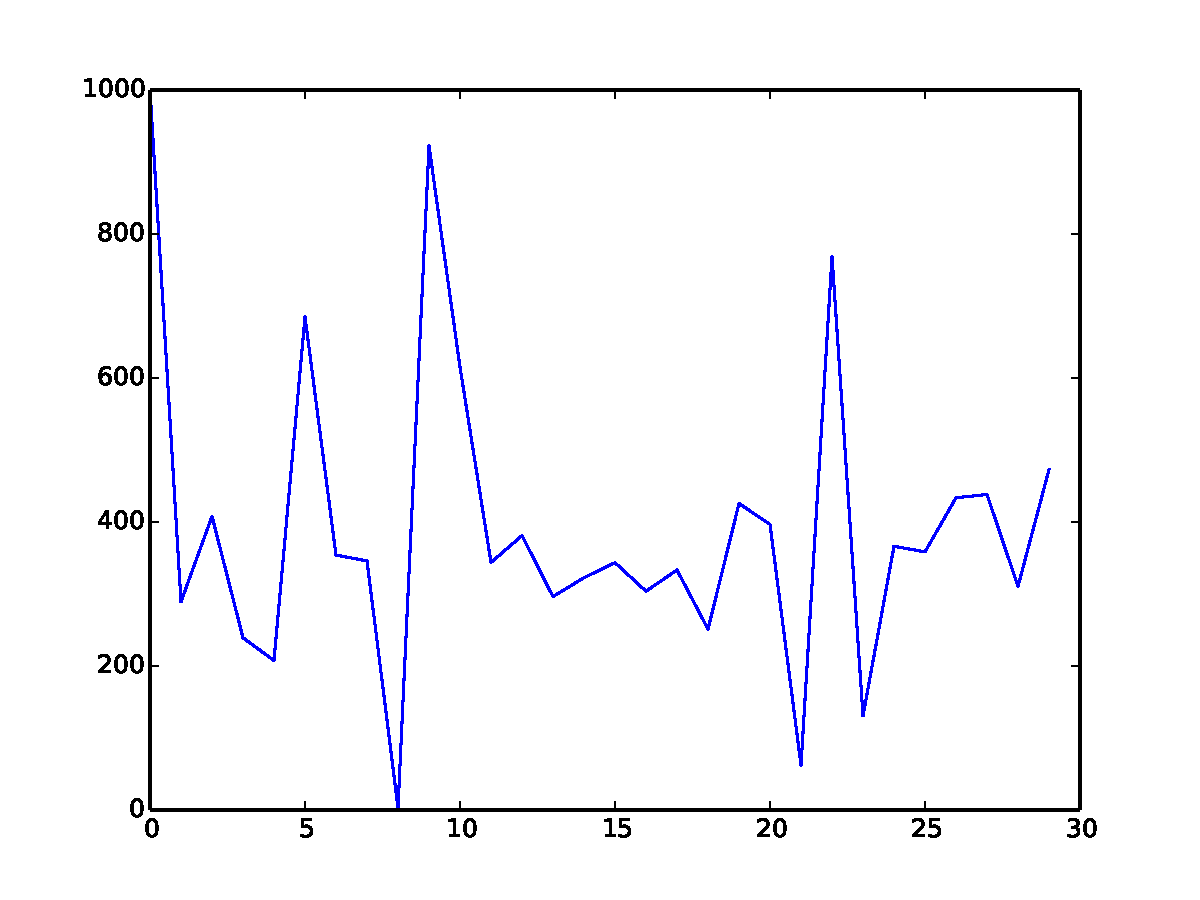
\includegraphics[width=0.97\linewidth]{/home/raphael/dissertation/bootstrap-filter/ESS_prior.pdf}
	\end{minipage}
	\caption{\textbf{(left)} Comparison of the expected value of the filtering distribution obtained using the prior proposal \textbf{(green)} simulated states \textbf{(blue)}. \textbf{(right)} The corresponding ESS. }
	\label{fig:prior}
\end{figure}

\begin{figure}[htb]
	\centering
	\begin{minipage}{.45\textwidth}
		\centering
		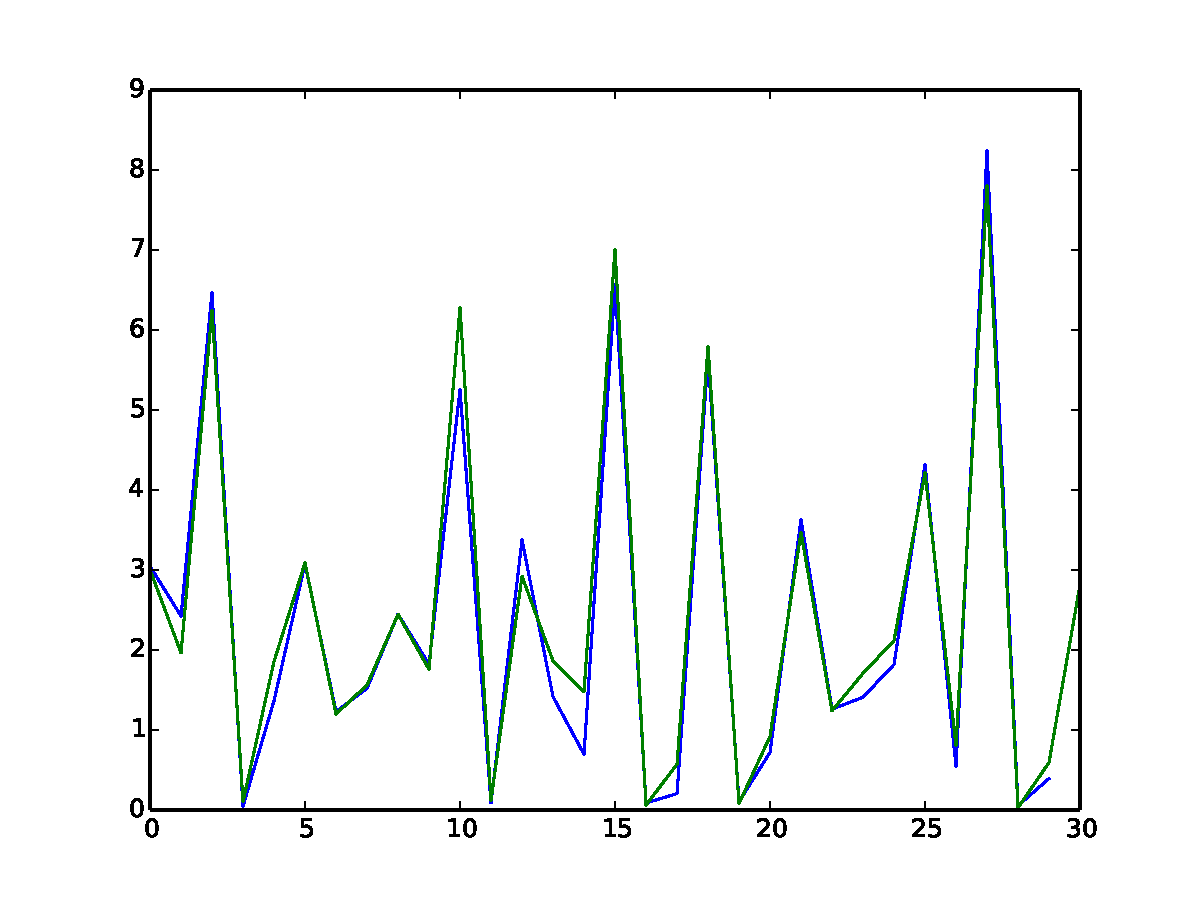
\includegraphics[width=0.97\linewidth]{bootstrap-filter/diagno_gamma.pdf}
	\end{minipage}
	\begin{minipage}{.45\textwidth}
		\centering
		
\includegraphics[width=0.97\linewidth]{bootstrap-filter/ESS_gamma.pdf}
	\end{minipage}
	\caption{\textbf{(left)} Comparison of the expected value of the filtering distribution obtained using the gamma proposal \textbf{(green)} simulated states \textbf{(blue)}. \textbf{(right)} The corresponding ESS. }
	\label{fig:gamma}
\end{figure}

\end{document}
